\documentclass[11pt,a4paper]{article}

\usepackage[margin=2.3cm]{geometry}
\usepackage{booktabs}
\usepackage{graphicx}
\usepackage{float}
\usepackage{amsmath}
\usepackage{amssymb}
\usepackage{array}
\usepackage{tabularx}
\usepackage{xcolor}
\usepackage{microtype}
\usepackage[hidelinks]{hyperref}

\newcommand{\ap}{\mathrm{AP}}
\newcommand{\code}[1]{\texttt{#1}}
\newcolumntype{Y}{>{\raggedright\arraybackslash}X}

\title{Fraud Detection on Highly Imbalanced Transaction Data\\
\large Temporal Validation, Feature Engineering, Ensemble Learning, and Deep Tabular Models}
\author{Vahid}
\date{\today}

\begin{document}

\maketitle

\begin{abstract}
This report presents a fraud-detection pipeline developed for highly imbalanced, chronologically ordered card transactions. The work compares gradient-boosted trees, imbalance-aware ensembles, FT-Transformer, and TabM under a shared temporal evaluation protocol. The main contributions are: (i) causal time, geographic, and card-history features; (ii) training-fold-only sampling and class weighting; (iii) validation-based selection of feature, sampling, model, and hyperparameter configurations; and (iv) a two-stage deep-learning procedure that selects the epoch count on temporal validation data before refitting on the complete training period. Across the completed experiments, XGBoost with all feature groups and random over-sampling achieved the highest validation average precision (0.9753), while CatBoost obtained a slightly higher final test average precision (0.9525). FT-Transformer substantially outperformed TabM among the deep models, reaching 0.9391 validation average precision and 0.8973 test average precision with focal loss. The results show that temporal and behavioral context contributes more than geographic features alone and that tree ensembles remain particularly effective for this dataset.
\end{abstract}

\section{Problem Definition}

The task is binary transaction classification: for each transaction $i$, predict a fraud label $y_i\in\{0,1\}$. The main difficulty is severe class imbalance. In the provided training file only 7,506 of 1,296,675 transactions are fraudulent (0.579\%); in the test file 2,145 of 555,719 are fraudulent (0.386\%). Consequently, accuracy is not an appropriate selection metric. A classifier that predicts every transaction as legitimate would exceed 99\% accuracy while detecting no fraud.

I therefore used \emph{average precision} (AP) as the primary validation metric. AP summarizes the precision--recall curve and emphasizes ranking quality for the rare positive class:
\begin{equation}
    \ap = \sum_n (R_n-R_{n-1})P_n,
\end{equation}
where $P_n$ and $R_n$ are precision and recall at threshold $n$. ROC-AUC is also reported on the final test period, but it is not used for configuration selection.

\section{Data and Evaluation Design}

\subsection{Chronological structure}

The data consists of two predefined chronological files (Table~\ref{tab:data}). The final training timestamp precedes the first test timestamp, so the files form a natural future holdout.

\begin{table}[H]
\centering
\caption{Dataset summary.}
\label{tab:data}
\begin{tabular}{lrrrrl}
\toprule
Split & Transactions & Fraud & Fraud rate & Cards & Date range \\
\midrule
Train & 1,296,675 & 7,506 & 0.579\% & 983 & Jan. 2019--Jun. 2020 \\
Test  &   555,719 & 2,145 & 0.386\% & 924 & Jun. 2020--Dec. 2020 \\
\bottomrule
\end{tabular}
\end{table}

For model development, I sorted \code{fraudTrain.csv} by transaction time and used its latest 20\% as validation data. The earlier 80\% was used to fit candidate configurations. This simulates deployment more faithfully than a random split because validation transactions occur after fitting transactions. After selection, the chosen pipeline is refitted on all of \code{fraudTrain.csv} and evaluated once on \code{fraudTest.csv}.

Exploratory analysis also showed that 99.97\% of test rows have a \code{(first,last)} pair observed in training. This is not label leakage by itself; it means the benchmark primarily evaluates future transactions of known customers. It does, however, mean that the result should not be interpreted as performance on unseen customers. Such a question would require an additional group split by \code{cc\_num}.

\subsection{Leakage controls}

The implementation applies the following controls:
\begin{itemize}
    \item the test period must begin after the training period;
    \item preprocessing is fitted inside the training pipeline;
    \item external sampling is applied only to training folds;
    \item card-history variables use shifted or cumulative prior values;
    \item the current transaction is removed from its own historical amount mean;
    \item validation and test labels are never used to generate features;
    \item model and hyperparameter selection uses validation AP, not test AP.
\end{itemize}

Earlier test transactions may contribute to history features for later test transactions, which matches an online scoring setting in which past observed transactions are available. No test label is used in this process.

\section{Feature Engineering}

I organized the features into five experimental strategies: \code{base}, \code{time}, \code{geo}, \code{behavioral}, and \code{all}. This made it possible to test not only the predictive model but also the source of predictive information.

\subsection{Base features}

The base strategy includes merchant, transaction category, gender, state, and job as categorical variables. Numerical variables include amount, city population, age at transaction time, $\log(1+\mathrm{amount})$, and a round-amount indicator.

The logarithmic transform compresses the long-tailed amount distribution while preserving order. The round-amount feature is motivated by the possibility that manually chosen fraudulent amounts have different decimal patterns from ordinary purchases. Age is computed at the transaction timestamp instead of using a fixed reference date.

\subsection{Time features}

The time group adds hour, day of week, month, and a weekend indicator. Fraud patterns can be time-dependent: an otherwise normal transaction can become suspicious when it occurs at an unusual hour or during a period inconsistent with ordinary customer activity. Month also captures slow temporal changes and seasonality.

\subsection{Geographic features}

The geographic group contains customer and merchant coordinates, their Haversine distance, an indicator for a very large customer-to-merchant distance, and distance from the previous merchant location. For two latitude--longitude points, the Haversine distance is
\begin{equation}
d=2R\arcsin\!\left(\sqrt{\sin^2\!\left(\frac{\Delta\phi}{2}\right)+
\cos\phi_1\cos\phi_2\sin^2\!\left(\frac{\Delta\lambda}{2}\right)}\right),
\end{equation}
where $R=6371.0088$ km. The intuition is that an implausible merchant location or a large jump between consecutive purchases can indicate compromised-card usage.

\subsection{Behavioral history features}

The behavioral group adds the prior card transaction count, observed card age, time since the previous transaction, amount-to-previous-amount ratio, and amount-to-historical-mean ratio. These variables transform a transaction from an isolated observation into a deviation from the card's past behavior. For example,
\begin{equation}
r_i=\frac{a_i}{\frac{1}{i-1}\sum_{j<i}a_j},
\end{equation}
compares the current amount $a_i$ with the mean of strictly earlier amounts for the same card. Large ratios can expose spending changes even when the absolute amount is not globally extreme.

The \code{all} strategy combines all groups. Categorical variables are one-hot encoded for classical models; numerical variables are standardized. Deep models instead use categorical embedding indices with an explicit unknown category and train-fitted numerical standardization.

\section{Models and Imbalance Handling}

\subsection{Ensemble models}

I evaluated XGBoost, CatBoost, LightGBM, EasyEnsemble, and RUSBoost in the completed runs. Random Forest is implemented in the framework, although no completed Random Forest metrics were present when this report was generated. Gradient-boosted trees are strong tabular baselines because they capture nonlinear feature interactions and are relatively insensitive to monotonic transformations.

Four external sampling settings were considered: no resampling, random under-sampling, random over-sampling, and SMOTE. Resampling is an imbalanced-learn pipeline step, so it is applied only after the temporal training fold has been selected. When external resampling is absent, class weights are derived from the training class ratio. EasyEnsemble and RUSBoost perform random under-sampling internally; combining them with an external sampler was therefore prohibited.

\subsection{Deep tabular models}

FT-Transformer maps each numerical variable to a token, embeds each categorical variable, prepends a learnable classification token, and processes the sequence with Transformer encoder layers. The default architecture uses token dimension 64, three layers, eight attention heads, GELU activation, and dropout 0.1.

TabM creates an efficient ensemble of $k=16$ MLP-style members within one model. Member probabilities are averaged for evaluation. Both models are trained with AdamW and support three imbalance-aware objectives:
\begin{enumerate}
    \item weighted binary cross-entropy (BCE);
    \item focal loss with $\alpha=0.95$ and $\gamma=2$;
    \item weighted BCE plus deviation loss.
\end{enumerate}

For the combined objective,
\begin{equation}
\mathcal{L}=\mathcal{L}_{\mathrm{weighted\ BCE}}+\lambda\mathcal{L}_{\mathrm{dev}}.
\end{equation}
The raw anomaly score is standardized against Gaussian reference samples. Normal observations are penalized by $|z|$, while fraud observations use $\max(0,m-z)$ with margin $m=5$. The goal is to keep normal scores near the reference mean and push fraud scores beyond the margin. I treated $\lambda$ as a tunable relative weight rather than assuming that the paper default transfers perfectly to this dataset.

\section{Hyperparameter Tuning}

\subsection{Classical models}

Each complete tuple
\[
(\text{model},\text{feature strategy},\text{sampling strategy})
\]
is treated as a candidate configuration. For each tuple, \code{RandomizedSearchCV} samples 10 hyperparameter combinations and evaluates them on a \code{PredefinedSplit}: earlier training rows have fold value $-1$, while the latest 20\% form the single validation fold. The scorer is \code{average\_precision}. This design preserves time order and ensures that preprocessing and sampling are re-fitted using only the fitting interval.

Table~\ref{tab:space} summarizes the important search dimensions.

\begin{table}[H]
\centering
\caption{Main randomized-search spaces for ensemble models.}
\label{tab:space}
\small
\begin{tabularx}{\textwidth}{lY}
\toprule
Model & Hyperparameter candidates \\
\midrule
XGBoost & Trees $\{200,400,700\}$; depth $\{4,6,8,12\}$; learning rate $\{0.02,0.05,0.1\}$; row and column subsampling $\{0.7,0.85,1.0\}$ \\
CatBoost & Trees $\{200,400,700\}$; depth $\{4,6,8,12\}$; learning rate $\{0.02,0.05,0.1\}$; L2 leaf regularization $\{1,3,5,9\}$ \\
LightGBM & Trees $\{200,400,700\}$; depth $\{4,6,8,12\}$; leaves $\{15,31,63\}$; learning rate and subsampling parameters \\
Random Forest & Trees and depth as above; max features $\{\sqrt{p},\log_2p,0.5p\}$; minimum leaf size $\{1,2,5,10\}$ \\
EasyEnsemble & Balanced subsets $\{5,10,20,30\}$; AdaBoost estimators $\{25,50,100,200\}$; learning rate; replacement \\
RUSBoost & Estimators $\{50,100,200,400\}$; learning rate; tree depth $\{1,2,3,5\}$; minimum leaf size; replacement \\
\bottomrule
\end{tabularx}
\end{table}

The winning randomized-search estimator is automatically refitted on all training-file rows. In the broader search script, all candidate tuples are ranked by validation AP and only the winner is evaluated on the final test file.

\subsection{Deep models}

Deep learning uses a two-stage procedure. First, the preprocessor and model are fitted on the earlier 80\% of the training file. Early stopping monitors validation AP with patience five, and the epoch with highest AP determines the training duration. Second, I create a fresh preprocessor and fresh randomly initialized model, fit them on the entire training file for the selected number of epochs, and evaluate on the test file. This avoids selecting epochs using test performance while allowing the final model to use all pre-test observations.

The principal deep comparisons vary model, feature strategy, and loss. The standard runs use batch size 2,048, learning rate $10^{-4}$, maximum 30 epochs, and weight decay $10^{-5}$.

\section{Experimental Results}

At report-generation time, the experiment directory contained 52 ensemble runs and 22 deep-learning runs. Some configurations were repeated, so aggregate means describe the available experiments rather than a perfectly balanced factorial study.

\subsection{Best ensemble configurations}

Table~\ref{tab:ensemble} reports the best validation-selected run for each completed ensemble family. XGBoost obtained the highest validation AP, while CatBoost produced the highest test AP by a small margin. Because CatBoost's test advantage was observed only after validation-based selection, it should not be used retrospectively to replace the validation winner.

\begin{table}[H]
\centering
\caption{Best completed configuration per ensemble model, ranked by validation AP.}
\label{tab:ensemble}
\begin{tabular}{lllrrr}
\toprule
Model & Features & Sampling & Validation AP & Test AP & Test ROC-AUC \\
\midrule
XGBoost      & all & random over & 0.9753 & 0.9517 & 0.9988 \\
CatBoost     & all & none        & 0.9732 & \textbf{0.9525} & 0.9989 \\
LightGBM     & all & none        & 0.9694 & 0.9464 & 0.9988 \\
RUSBoost     & all & internal    & 0.8799 & 0.8480 & 0.9953 \\
EasyEnsemble & all & internal    & 0.7262 & 0.6479 & 0.9845 \\
\bottomrule
\end{tabular}
\end{table}

\begin{figure}[H]
\centering
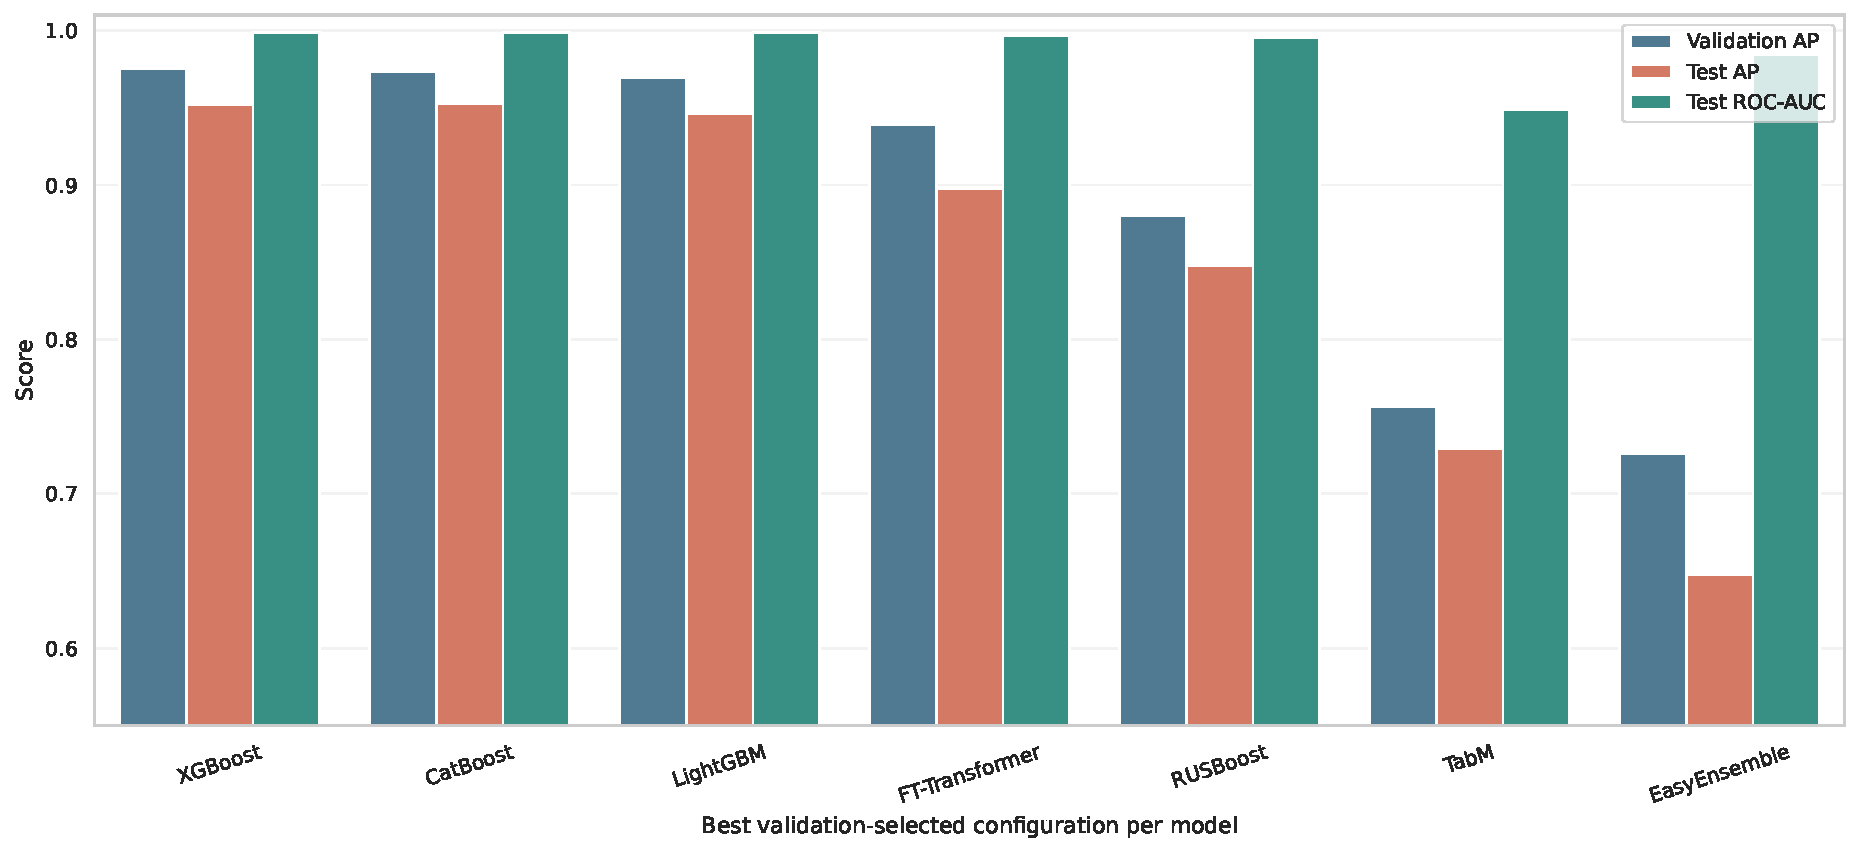
\includegraphics[width=\textwidth]{figures/best_model_comparison.pdf}
\caption{Validation AP, test AP, and test ROC-AUC for the best validation-selected configuration of each model. The high ROC-AUC values should be interpreted together with AP because fraud is rare.}
\label{fig:models}
\end{figure}

\subsection{Influence of feature engineering and sampling}

The \code{all} strategy had the highest ensemble mean validation AP (0.9311) and best AP (0.9753), followed by behavioral features (mean 0.9155). Time features were useful but weaker in isolation (mean 0.8658). Base and geographic strategies had substantially lower means (0.7273 and 0.7075). This supports the original intuition that fraud is best characterized by a combination of current-transaction attributes and deviations from historical card behavior.

Among models that use external sampling, random over-sampling had the highest mean validation AP (0.8677) and produced the best individual run. No external sampling was nearly identical on average (0.8650), indicating that class weighting alone was competitive. SMOTE and random under-sampling were weaker on average. These values are not pure causal estimates because model and feature coverage is not perfectly balanced; the individual points in Figure~\ref{fig:ensemble-influence} expose this variation.

\begin{figure}[H]
\centering
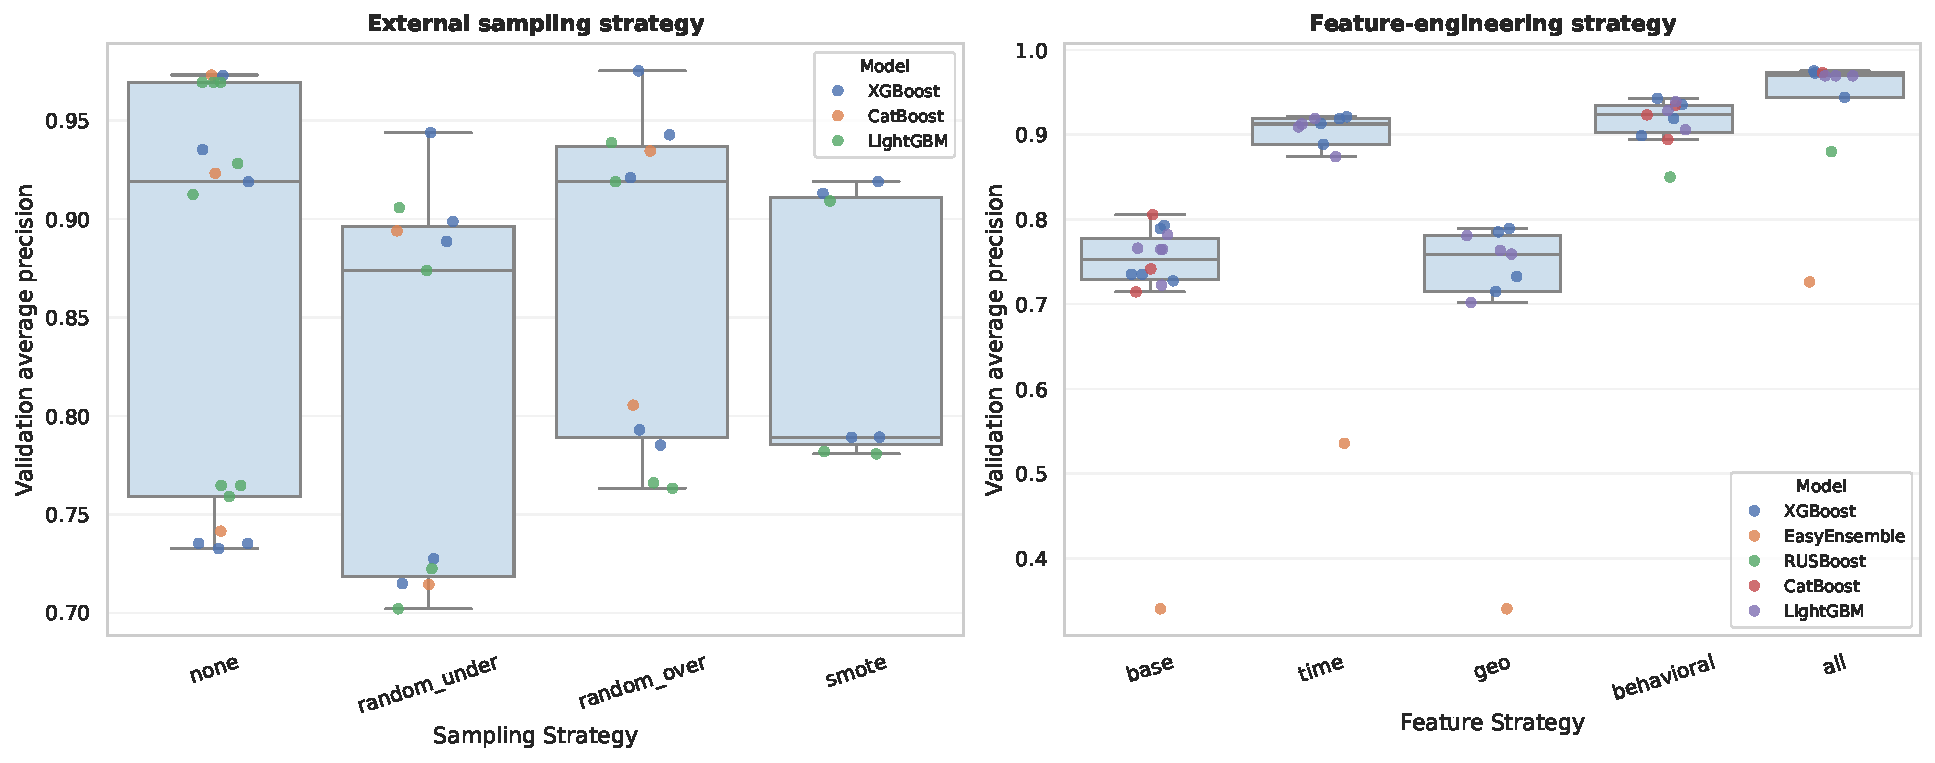
\includegraphics[width=\textwidth]{figures/ensemble_influence.pdf}
\caption{Validation AP across ensemble sampling strategies (left) and feature strategies (right). EasyEnsemble and RUSBoost are excluded from the external-sampling panel because their under-sampling occurs internally. Points are individual experiments and colors identify models.}
\label{fig:ensemble-influence}
\end{figure}

\subsection{SHAP values and feature importance}

I generated explainability outputs for a LightGBM experiment using all feature groups and no external sampling. This run reached 0.9694 validation AP, 0.9464 test AP, and 0.9988 test ROC-AUC, making it both a strong model and a representative candidate for interpretation.

Two complementary importance measures were used. LightGBM's native importance counts how often a feature is used to split trees. This measure is efficient but may favor continuous or high-cardinality variables that offer many potential split points. SHAP instead attributes the change in model output to each feature for each evaluated transaction. Global SHAP importance is the mean absolute attribution,
\begin{equation}
I_j^{\mathrm{SHAP}}=\frac{1}{N}\sum_{i=1}^{N}|\phi_{ij}|,
\end{equation}
where $\phi_{ij}$ is the SHAP value of feature $j$ for transaction $i$.

Table~\ref{tab:importance} shows the leading variables under both definitions. Transaction amount is dominant in both. More importantly for the feature-engineering argument, amount relative to the previous transaction, transaction sequence number, hour, and time since the previous transaction all appear near the top. The model therefore uses both the current transaction and its temporal/card-history context.

\begin{table}[H]
\centering
\caption{Leading LightGBM features according to mean absolute SHAP value and native split importance.}
\label{tab:importance}
\small
\begin{tabular}{lrlr}
\toprule
Feature (SHAP ranking) & Mean $|\phi|$ & Feature (native ranking) & Splits \\
\midrule
Amount & 0.703 & Amount & 3,116 \\
Card transaction number & 0.444 & Amount / previous amount & 2,631 \\
Gas-transport category & 0.398 & Hour & 1,838 \\
Amount / previous amount & 0.379 & Hours since previous transaction & 1,655 \\
Hour & 0.371 & Customer age & 1,518 \\
Shopping-POS category & 0.333 & Log amount & 1,234 \\
Entertainment category & 0.296 & Card transaction number & 1,193 \\
Hours since previous transaction & 0.288 & Amount / historical mean & 1,193 \\
\bottomrule
\end{tabular}
\end{table}

\begin{figure}[H]
\centering
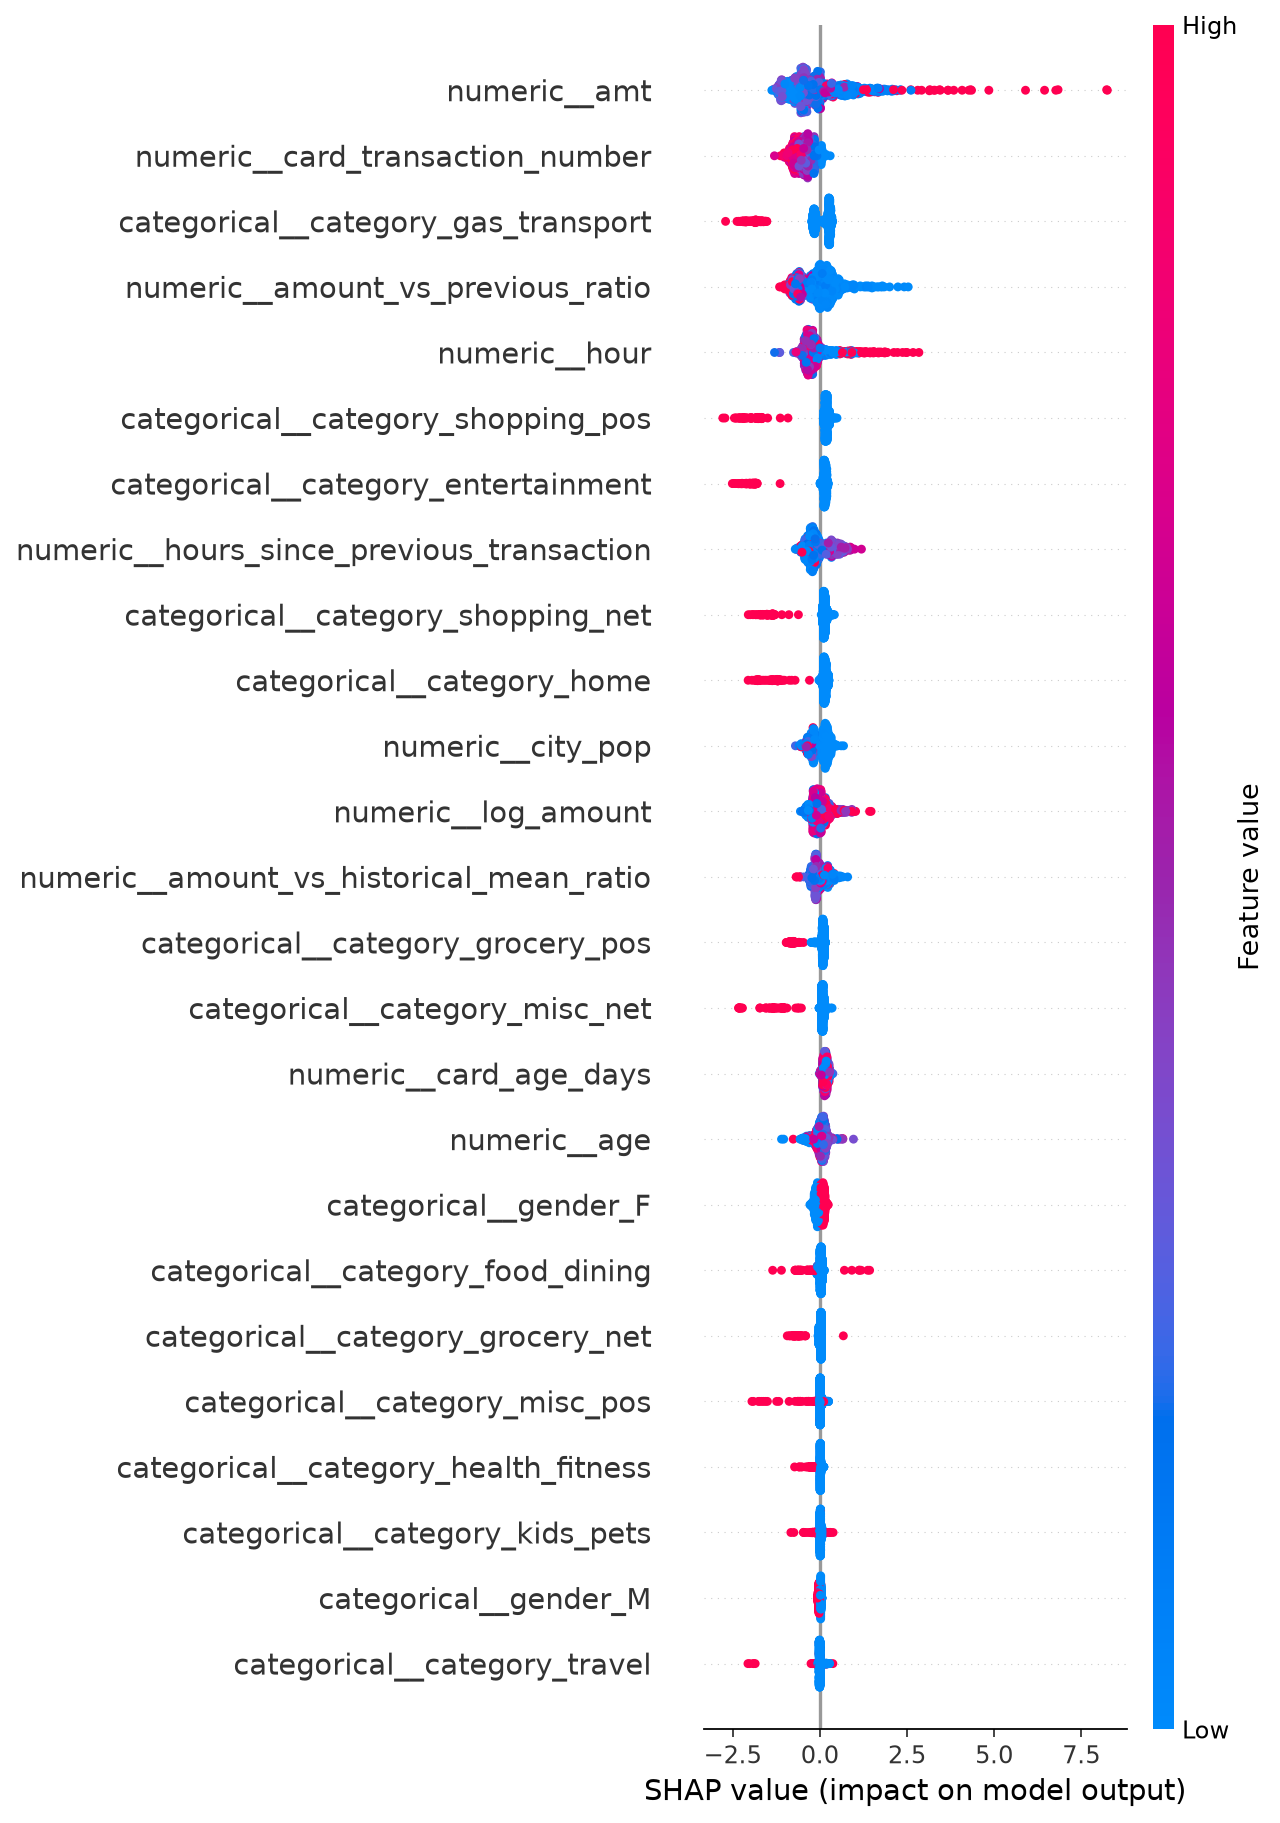
\includegraphics[width=0.70\textwidth]{figures/lightgbm_shap_summary.png}
\caption{SHAP beeswarm for the explained LightGBM run. Features are ordered by mean absolute SHAP value. Horizontal position is the contribution to the model output; color represents the observed feature value. Each point is one sampled test transaction.}
\label{fig:shap}
\end{figure}

Figure~\ref{fig:shap} provides direction as well as magnitude. High transaction amounts generally push the output strongly toward fraud. Later hour values and long times since the previous transaction also tend to increase the fraud score. Several transaction-category indicators have large negative attributions when present, showing that category affects not only importance but also the direction of the prediction. The amount-to-previous ratio has a nonlinear pattern, so it should not be summarized as a simple monotonic rule.

\begin{figure}[H]
\centering
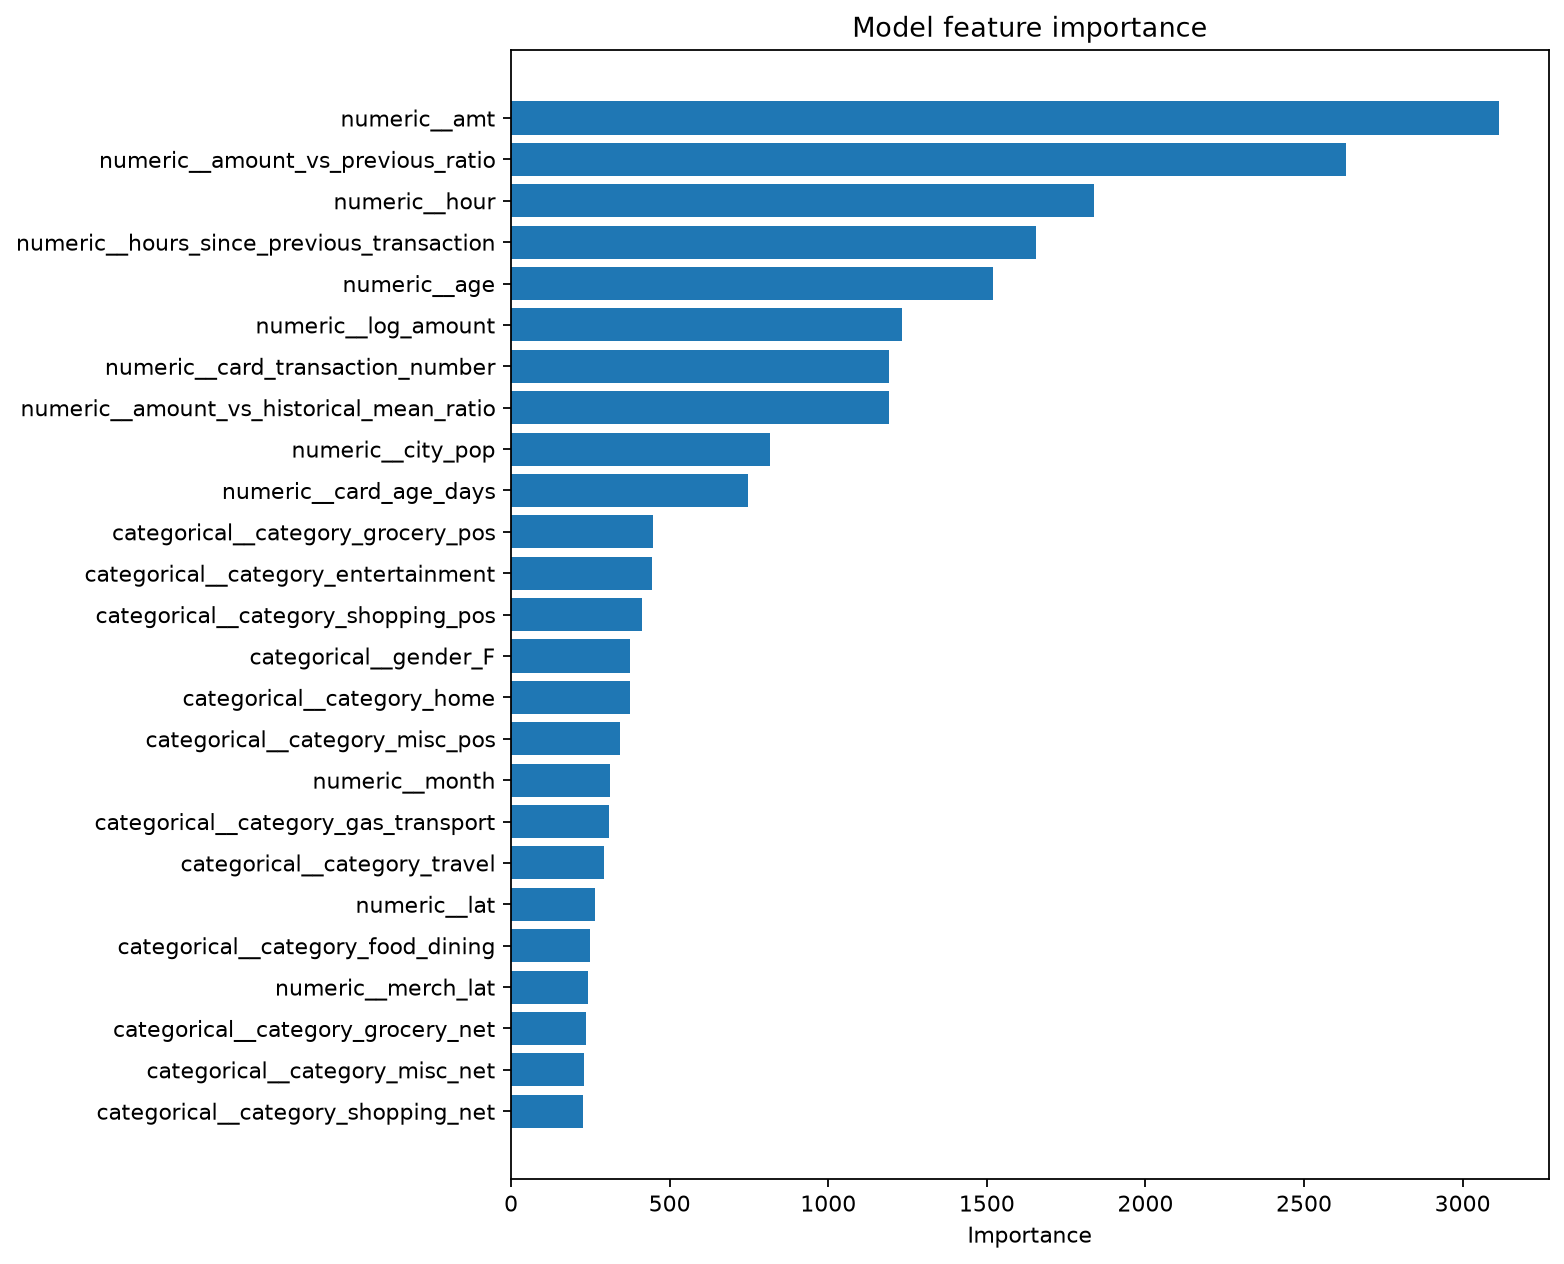
\includegraphics[width=0.88\textwidth]{figures/lightgbm_feature_importance.png}
\caption{Native LightGBM split importance for the same experiment. Agreement with SHAP on amount and several behavioral features increases confidence that these variables materially influence this fitted model.}
\label{fig:native-importance}
\end{figure}

These explanations describe associations learned by one fitted model; they are not causal effects. Correlated features such as amount and log amount can share or redistribute importance, and one-hot category indicators are interpreted relative to their omitted alternatives. SHAP values were computed on a reproducible sample of at most 1,000 test rows to keep the analysis tractable.

\subsection{Deep-learning results}

FT-Transformer clearly outperformed TabM in the completed experiments (Table~\ref{tab:deep}). Focal loss selected 26 epochs and achieved the highest FT-Transformer validation AP. The deviation-regularized run had slightly lower validation AP but slightly higher test AP; this again should not override validation-based selection.

\begin{table}[H]
\centering
\caption{Best validation-selected configuration per deep model.}
\label{tab:deep}
\begin{tabular}{lllrrrr}
\toprule
Model & Features & Loss & Epochs & Validation AP & Test AP & Test ROC-AUC \\
\midrule
FT-Transformer & all  & focal                  & 26 & 0.9391 & 0.8973 & 0.9963 \\
TabM           & time & weighted BCE + deviation & 20 & 0.7565 & 0.7294 & 0.9487 \\
\bottomrule
\end{tabular}
\end{table}

Across deep runs, \code{all} had the highest mean validation AP (0.7731), followed by time (0.6601). The combined weighted-BCE-plus-deviation objective had the highest mean across available runs (0.6732), whereas focal loss produced the best individual run (0.9391). Part of the aggregate loss difference is explained by model and feature composition, so the controlled comparison within FT-Transformer with all features is more informative: focal (0.9391), combined deviation loss (0.9331), and weighted BCE (0.9066).

\begin{figure}[H]
\centering
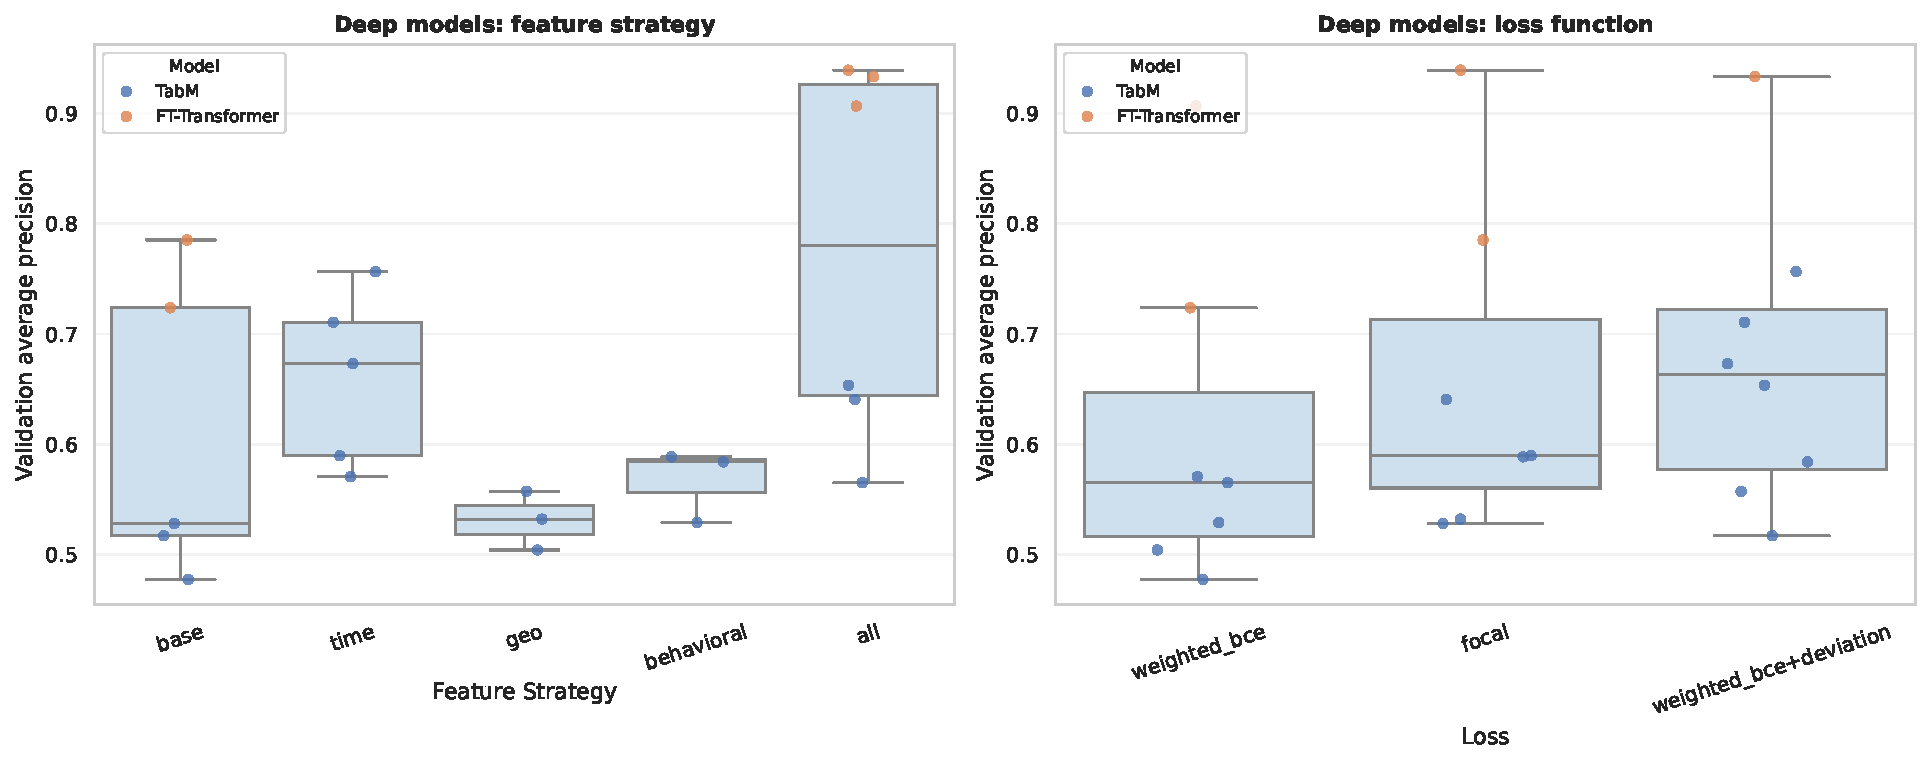
\includegraphics[width=\textwidth]{figures/deep_influence.pdf}
\caption{Validation AP of deep-learning experiments by feature strategy (left) and loss (right). Points show individual experiments; distributions should be read with the number and identity of models in each group in mind.}
\label{fig:deep-influence}
\end{figure}

\subsection{Validation and test consistency}

Figure~\ref{fig:val-test} shows that validation and test AP are strongly related, although test AP is often lower. This is expected under temporal distribution shift: the fraud prevalence changes from 0.579\% in training to 0.386\% in testing, and transaction behavior may also evolve. The result reinforces the importance of temporal rather than random validation.

\begin{figure}[H]
\centering
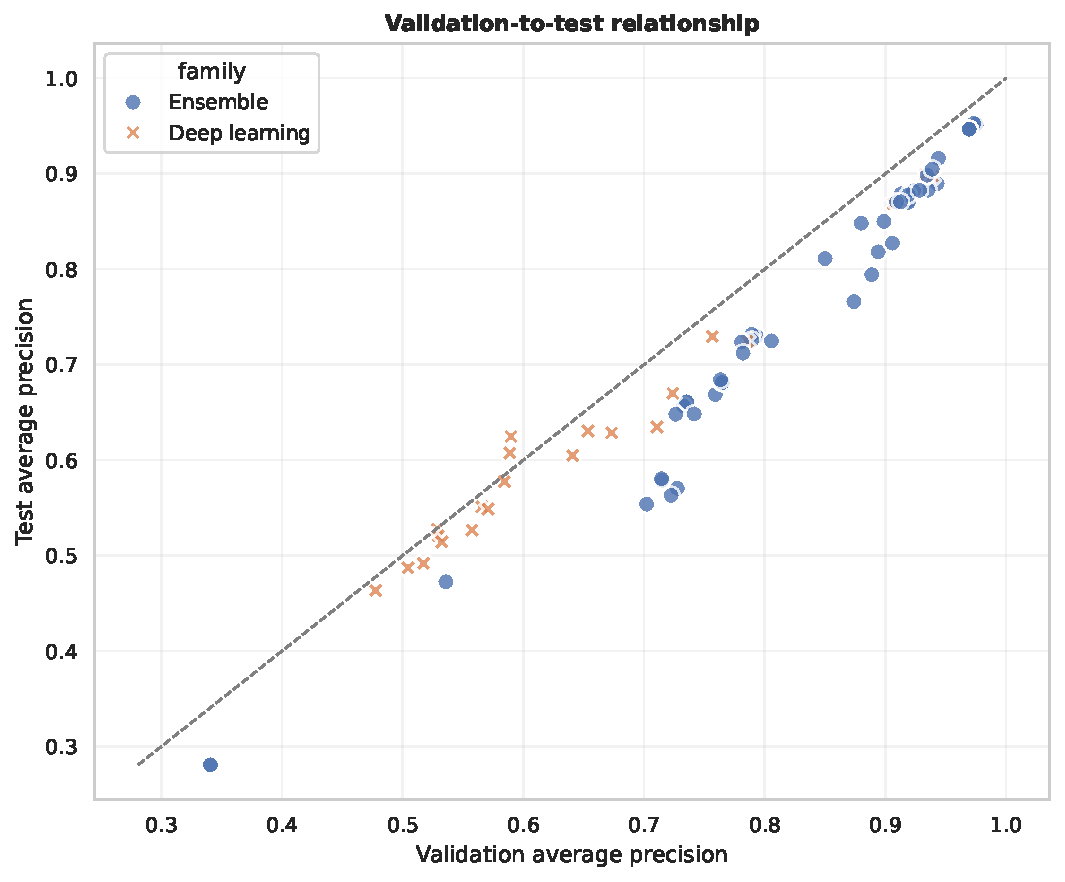
\includegraphics[width=0.72\textwidth]{figures/validation_test_relationship.pdf}
\caption{Relationship between validation and test average precision for completed experiments. The dashed line represents equal validation and test AP.}
\label{fig:val-test}
\end{figure}

\section{Discussion}

The strongest models were boosted trees with combined feature groups. This is consistent with the strengths of gradient boosting on heterogeneous tabular data: it can learn nonlinear thresholds such as unusual amount ratios at particular times without requiring a large neural representation-learning budget. FT-Transformer was competitive but remained below the top tree ensembles. TabM was less stable and more sensitive to feature and loss choices in the completed runs.

Behavioral and time features were more valuable than geographic features alone. A likely explanation is that absolute coordinates and customer-to-merchant distance are too coarse: legitimate travel can create large distances, while card-present fraud can occur locally. In contrast, amount ratios, recency, and transaction sequence position personalize the transaction relative to the card's own history.

The results also show why ROC-AUC cannot be the only metric. Several models have ROC-AUC near 0.999, but their AP values differ materially. AP reveals whether positive predictions remain precise when fraud prevalence is below one percent.

\section{Limitations and Future Work}

\begin{itemize}
    \item \textbf{Known-customer evaluation:} most test customers appear in training. A group-temporal split by \code{cc\_num} should be added to measure unseen-customer generalization.
    \item \textbf{Unequal experiment coverage:} repeated and incomplete combinations make aggregate means descriptive rather than causal. A balanced factorial experiment with several seeds would permit uncertainty estimates.
    \item \textbf{Threshold selection:} AP evaluates ranking, but deployment requires a threshold selected using business costs or an alert-budget constraint. Precision at fixed recall and recall at fixed alert rate should be reported.
    \item \textbf{Calibration:} class weighting and sampling can distort probability calibration. Platt scaling or isotonic calibration fitted on validation data could be studied.
    \item \textbf{Concept drift:} rolling or expanding-window validation would provide a stronger estimate across multiple time periods than one holdout boundary.
    \item \textbf{Deep tuning:} architecture dimensions, learning rate, deviation weight, and margin should be searched systematically rather than compared through a limited set of runs.
\end{itemize}

\section{Conclusion}

I implemented an end-to-end, leakage-aware fraud-detection framework that separates preprocessing, feature engineering, sampling, model construction, tuning, deep training, explanation, and experiment analysis. The key methodological choice was to select every configuration using a future validation segment and reserve the supplied test file for final evaluation.

Feature engineering had a large practical effect. Combining time, geographic, and especially behavioral history features raised validation AP well above the base-only alternatives. XGBoost with all features and random over-sampling was the validation winner at 0.9753 AP; CatBoost and LightGBM were close. FT-Transformer was the strongest neural model at 0.9391 validation AP, while TabM trailed substantially. Overall, the experiments demonstrate that careful temporal design and causal behavioral context matter at least as much as the choice of classifier for imbalanced transaction fraud detection.

\begin{thebibliography}{9}

\bibitem{fttransformer}
Y. Gorishniy, I. Rubachev, V. Khrulkov, and A. Babenko,
``Revisiting Deep Learning Models for Tabular Data,''
\emph{Advances in Neural Information Processing Systems}, 2021.

\bibitem{tabm}
Y. Gorishniy, I. Rubachev, and A. Babenko,
``TabM: Advancing Tabular Deep Learning with Parameter-Efficient Ensembling,''
arXiv preprint, 2024.

\bibitem{devnet}
G. Pang, C. Shen, and A. van den Hengel,
``Deep Anomaly Detection with Deviation Networks,''
\emph{Proceedings of the ACM SIGKDD International Conference on Knowledge Discovery and Data Mining}, 2019.

\bibitem{smote}
N. V. Chawla, K. W. Bowyer, L. O. Hall, and W. P. Kegelmeyer,
``SMOTE: Synthetic Minority Over-sampling Technique,''
\emph{Journal of Artificial Intelligence Research}, 2002.

\bibitem{easyensemble}
X.-Y. Liu, J. Wu, and Z.-H. Zhou,
``Exploratory Undersampling for Class-Imbalance Learning,''
\emph{IEEE Transactions on Systems, Man, and Cybernetics, Part B}, 2009.

\end{thebibliography}

\end{document}
